\documentclass[fleqn,11pt,aspectratio=169]{beamer}
\usetheme[freifunk]{stratum0}

\usepackage[utf8]{inputenc}
\usepackage[ngerman]{babel}
\usepackage{amsmath}
\usepackage{tikz}
\usepackage{etex}
\usepackage{multicol}
\usepackage{booktabs}
\usepackage{colortbl}
\usepackage{tabularx}
\usepackage{longtable}
\usepackage{pgfplots}
\usepackage[normalem]{ulem}


\title[Freifunk Braunschweig]{Freifunk Braunschweig}
\subtitle{Freies WLAN für Braunschweig}
\author[Kasa, Chrissi]{Kasa, Chrissi}
\date{\today}

\begin{document}

\begin{frame}[plain]
  \titlepage
\end{frame}


\section{Einleitung}

\begin{frame}{Wer sind wir?}
	\begin{multicols*}{2}
	\begin{block}{}
  \begin{itemize}
  	\item Gemeinnütziger Verein
		\item Gegründet 2011, heute 70 Mitglieder
		\item Keine Firma, müssen nichts verkaufen
		\item Warum machen wir das? Weil wir es können (wollen)
	\end{itemize}
	\end{block}
	\centering
	
\includegraphics{stratum0.pdf}
\end{multicols*}
\end{frame}

\begin{frame}{Was sind wir?}
	\begin{multicols*}{2}
	\begin{block}{}
  \begin{itemize}
		\item Nerds!
		\item Wilder Mix: Studenten, Arbeitende, Schüler, ...
		\item Plattform zum Austausch
		\item Raum für nerdige Treffen
	\end{itemize}
	\end{block}
	\centering
	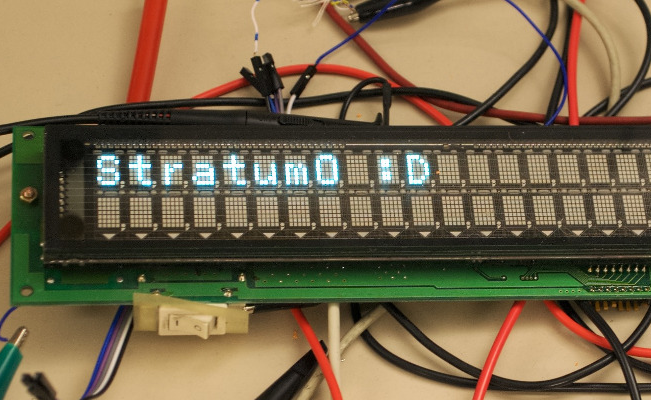
\includegraphics{stratum0_display.png}
\end{multicols*}
\end{frame}

\begin{frame}{Hacker?}
	\begin{multicols*}{2}
	\begin{block}{}
  \begin{itemize}
		\item Ein Hacker ist jemand, der versucht einen Weg zu finden, wie man mit einer Kaffeemaschine Toast zubereiten kann.\\ (Wau Holland)
	\end{itemize}
	\end{block}
	\centering
	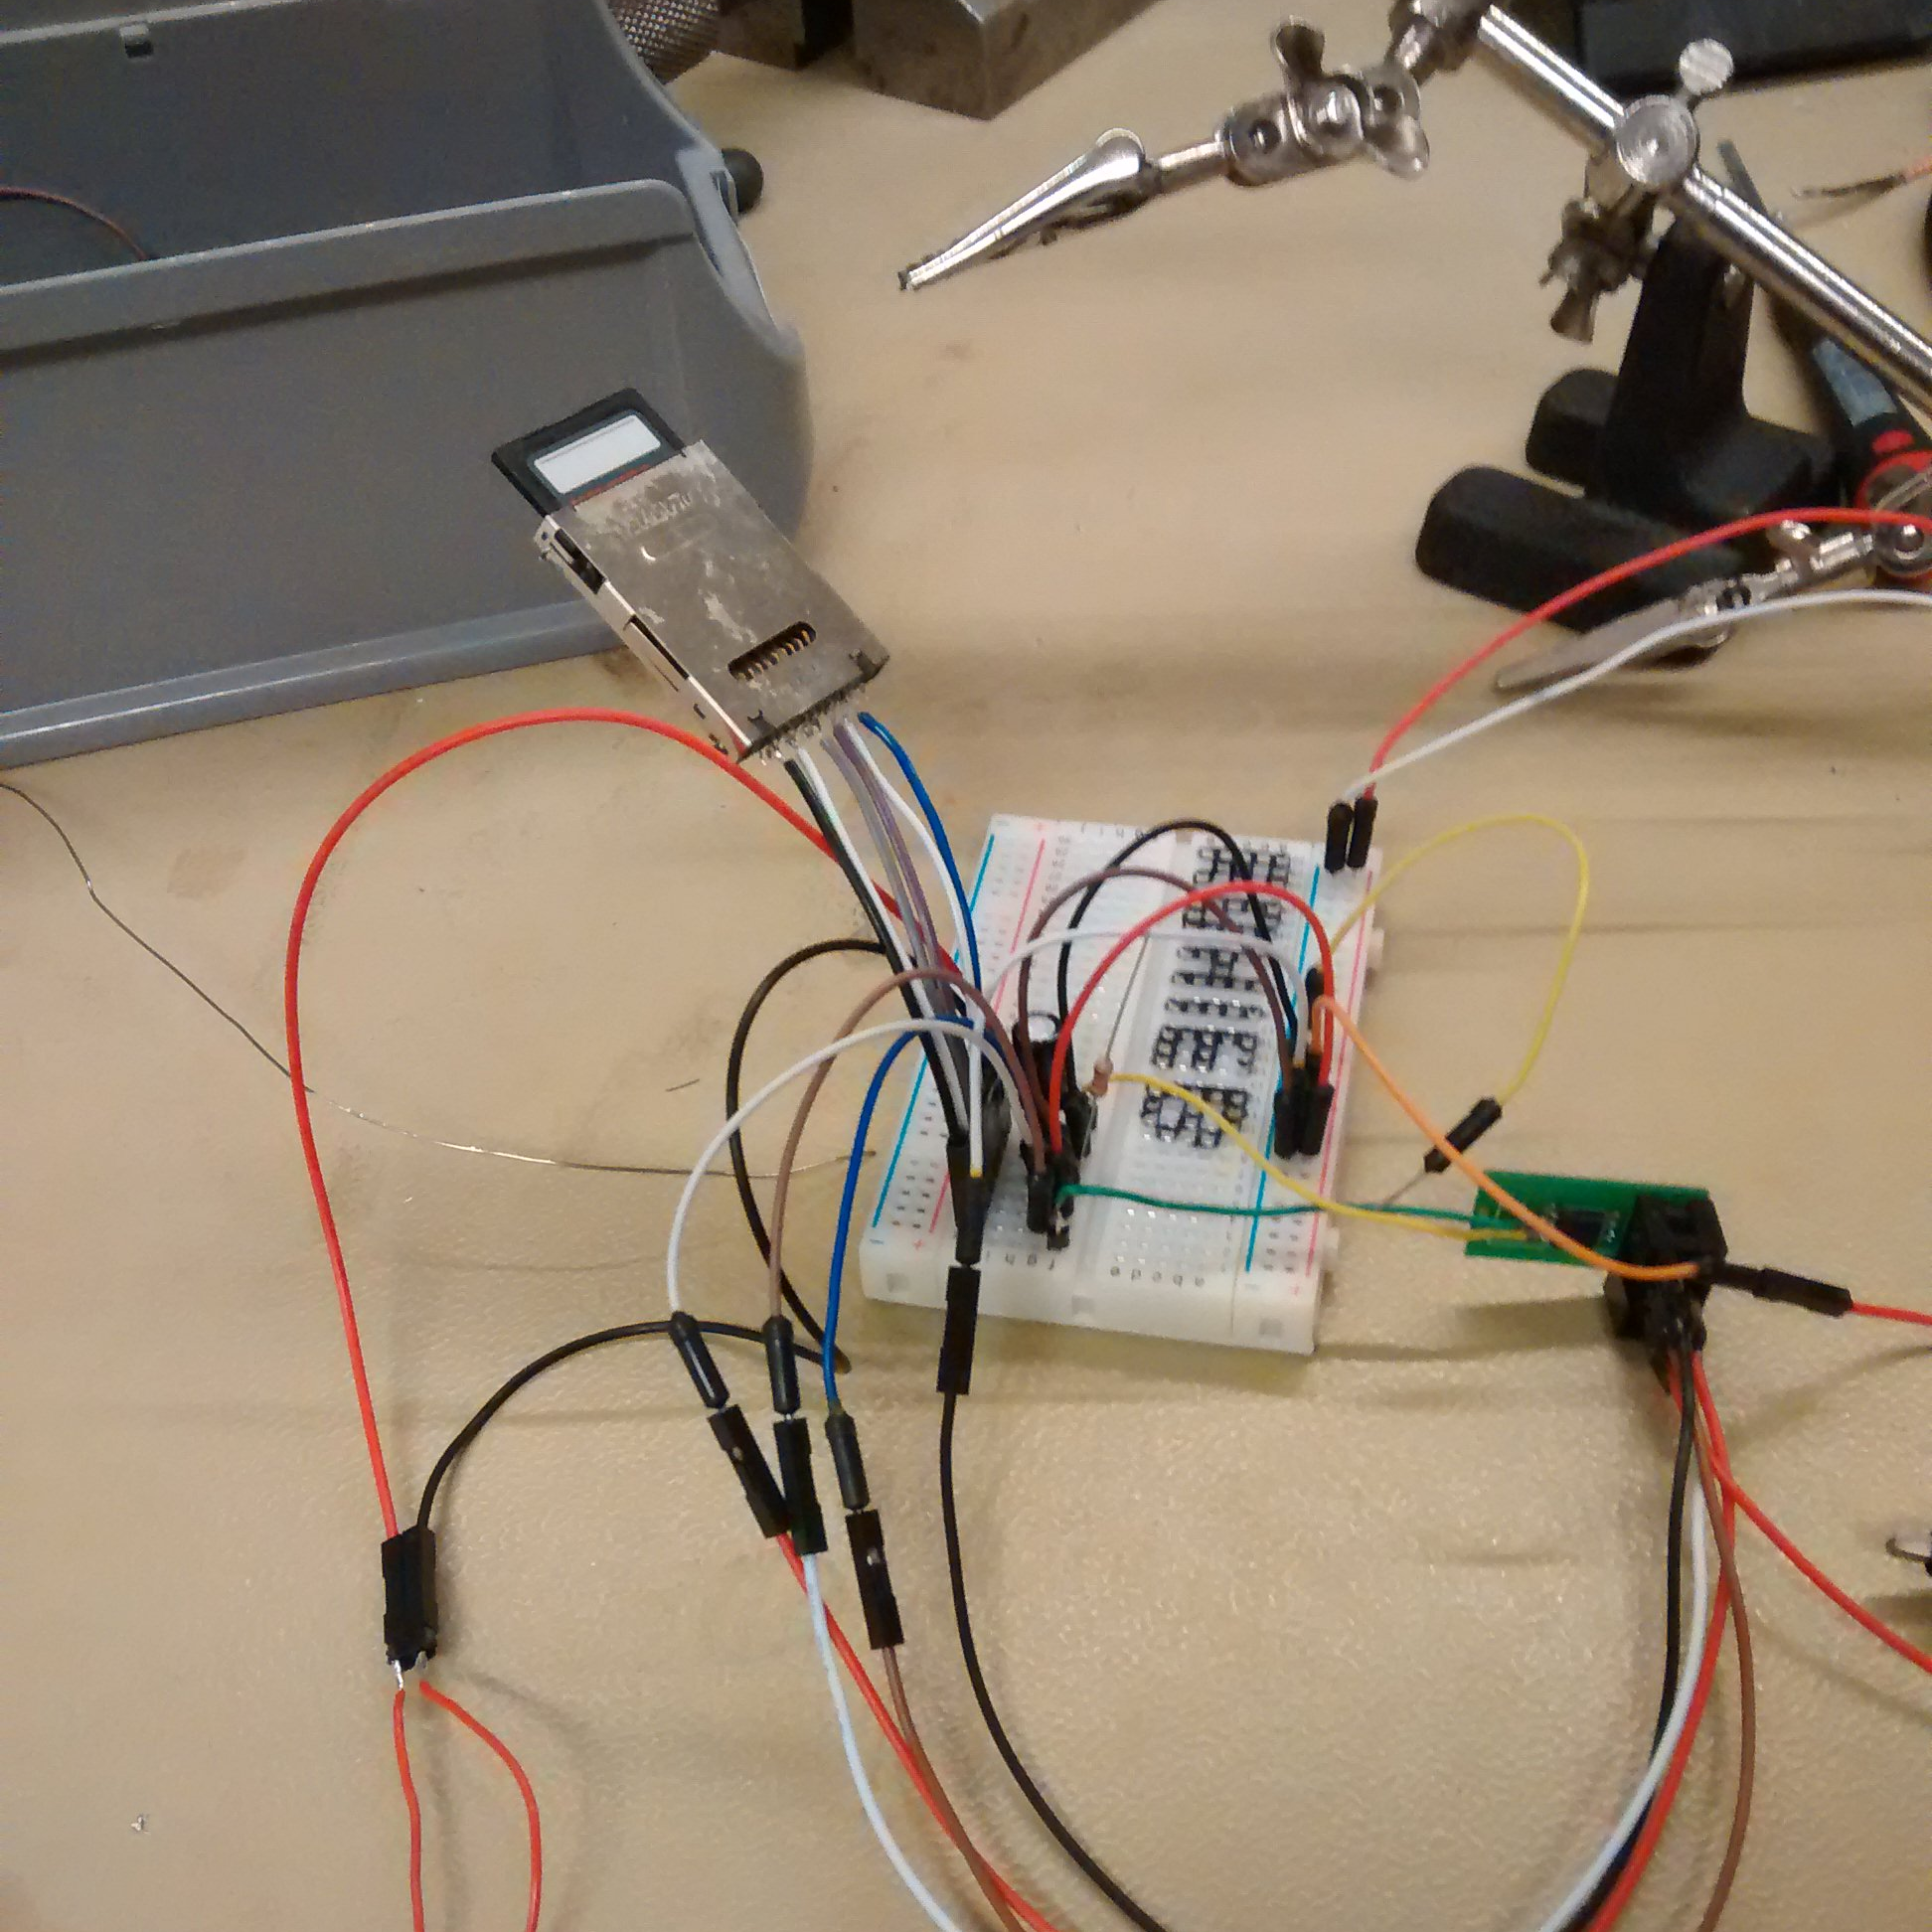
\includegraphics[height=0.9\textheight]{stratum0atmusic.png}
\end{multicols*}
\end{frame}



\begin{frame}{Projekte}
	\begin{multicols*}{2}
	\begin{block}{}
  \begin{itemize}
		\item CTF
		\item CoderDojo
		\item Kopter-Club Braunschweig
		\item Vortragsabende
		\item Freifunk Braunschweig
	\end{itemize}
	\end{block}
	\centering
	
\includegraphics[height=0.9\textheight]{coderdojo.pdf}
\end{multicols*}
\end{frame}

\begin{frame}{Freifunk: Geschichte}
	\begin{block}{}
  \begin{itemize}
		\item Beginn der Initiative: 2002 / 2003
		\item Ziele damals:
		\begin{itemize}
			\item Internet (in entlegende Gebiete) verteilen
			\item WLAN war die Ausnahme
			\item Technik war komplex
			\item Ausrichtung an Experten
		\end{itemize}
	\end{itemize}
	\end{block}
\end{frame}


\begin{frame}{Das Problem}
\begin{multicols*}{2}
\begin{block}{}
\begin{itemize}
		\item Weltweite Länder mit Störerhaftung:
		\pause
		\begin{itemize}
			\item Deutschland
			\pause
			\item Deutschland
			\pause
			\item Deutschland
			\pause
		\end{itemize}
	\end{itemize}
\end{block}
\centering
	
\includegraphics[width=0.5\textwidth]{neuland.jpg}
\end{multicols*}
\end{frame}

\picturetitleframe{Wie es sein sollte}{wasser.jpg}


\begin{frame}{Wie es sein sollte}
	\begin{itemize}
		\item	Grundrecht auf Zugang zu Informationen
		\pause
		\item unzensiert
		\pause
		\item datensparsam
		\pause
		\item Möglichkeit zur Anonymität
		\pause
		\item für Gäste kostenlos
		\pause
		\item geringe Zugangshürde
	\end{itemize}
\end{frame}

\picturetitleframe{Unsere Lösung}{./ffbs_router.png}

\begin{frame}{Warum ist unsere Lösung besser?}
\begin{itemize}
	\item Offenes WiFi
	\item Daten werden durch deine lokale Freifunk-Initiative umgeleitet
\end{itemize}
\end{frame}

\begin{frame}{Hacken!}
\begin{itemize}
	\item Technische Lösung für ein politisches Problem \textbackslash o/
	\item Die schlechte Nachricht: \\Die Störerhaftung gibt es immernoch - aber durch die Freifunk-Initiative getragen
	\pause
	\item Oder: Die Freifunk-Initiative sucht sich einen Dienstleister im Ausland...
\end{itemize}
\end{frame}

\begin{frame}{Politik}
\begin{itemize}
	\item Freifunker setzen sich für die Aufhebung der Störerhaftung ein 
	\pause
	\item Gerichtlich:
	\begin{itemize}
		\item Freifunk Berlin vor dem AG Charlottenburg (2014)
		\item AG Hamburg (2014)
		\item Ziel: Feststellung, dass das Providerprivileg (§8 TMG) auch für Freifunker gilt
		\item Es gibt hierzu noch keine höchstrichterliche Entscheidung
	\end{itemize}
	\pause
	\item Organisatorisch:
	\begin{itemize}
		\item Wenn man ein Provider sein muss, um in den Genuss des Providerprivilegs zu kommen, dann werden wir halt Provider!
		\item Freifunk Rheinland ist beim RIPE registriert und gilt damit technisch als Provider 
		\item Jede lokale Initiative kann deren Dienst nutzen, um ebenfalls Provider zu sein
	\end{itemize}
\end{itemize}
\end{frame}

\begin{frame}{Landespolitik}
  \begin{itemize}
    \item Entschließungsantrag SPD, Bündnis 90/Die Grünen, 03.11.2015, Drucksache 17/4524: \\
    Freies WLAN in Niedersachsen: Freifunk unterstützen, Bürgernetze ausbauen!
    \item Förderung von Freifunk und von Bürgern betriebenen Netzen durch 
    \begin{itemize} 
      \item finanzielle und 
      \item politische Unterstützung, sowie
      \item gezielte Information über / für Freifunk an die Kommunen.
    \end{itemize}
    \item Erstes Treffen zwischen Landespolitik (Belit Onay (Grüne), Maximilian Schmidt (SPD)) und Freifunk-Gruppen aus NDS am 10.02.2016
    \item Zweite Beratung Plenarprotokoll17/91 (Tagesordnung) 08.03.2016 
  \end{itemize}
\end{frame}

\begin{frame}{Freifunk: Heute}
	\begin{multicols*}{2}
	\begin{block}{}
  \begin{itemize}
		\item Dachverband Freie Netze e.V.
		\item 274 Initiativen
		\item 28.700 Zugangspunkte
		\item Grob geschätzt: über 300.000 Nutzer
	\end{itemize}
	\end{block}
	\centering
	
\includegraphics[height=0.9\textheight]{freifunk.png}
	\end{multicols*}
\end{frame}

\begin{frame}{Warum tun wir das?}
\begin{itemize}
	\item Wir mögen überall offenes WLAN !
	\item Weil es sonst keiner so tut, wie wir es haben wollen
	\begin{itemize}
		\item Kommerzielles WLAN ist von Unternehmen gemacht, die Gewinn erwirtschaften müssen
		\item Freifunk machen wir so, wie wir es haben wollen
	\end{itemize}
	\item Weil wir es können wollen
	\item Wir kennen uns mit Technik aus und wollen das mit anderen teilen
	\item \textit{For fun and \sout{profit}}
\end{itemize}
\end{frame}

\begin{frame}{Mitmachen}
\begin{itemize}
	\item Freifunk nutzen 
	\pause
	\item Knoten betreiben (lassen)
	\pause
	\item Weiter erzählen
	\pause
	\item Mithelfen\\
	Jeden Mittwoch 19.00 Uhr im Stratum 0
\end{itemize}
\end{frame}

\begin{finalframe}{}
Kasa <kasa@stratum0.org>\\
Chrissi <chris@tinyhost.de>\\
\end{finalframe}

\end{document}
